\chapter{Magma Dynamics: porosity waves}
\label{cha:porosity-waves}

\section{Problem Overview}
\label{sec:porosity_waves-formulation}


While many modeling packages in Earth science solve for thermal or
thermo-chemical convection,  one of the strengths of \TF{} is that it
is not a ``convection code'', but rather a general finite element PDE
solver and can be used to model arbitrary problems as long as the weak
forms are well posed.  In particular,  \TF{} was primarily designed to
explore coupled fluid/solid mechanics with a primary application area
being the flow of magma and fluids in the deep earth.  A more general
theory of magma dynamics has been derived by multiple authors
\cite{mckenzie_generation_1984,scott_magma_1984,scott_magma_1986,spiegelman_flow_1993,spiegelman_flow_1993-1,bercovici_two-phase_2001-1,bercovici_energetics_2003,simpson_multiscale_2010,simpson_multiscale_2010-1}
that considers the flow of a low viscosity fluid in a viscously
deformable solid matrix.  From the beginning of magma dynamics,  one
of the intriguing features of these models is that they admit
dispersive non-linear magmatic
solitary  waves that propagate through the solid as ``hump
shaped'' blobs with radial symmetry that propagate at a characteristic
speed $c$ that depends on amplitude, dimension and material
parameters.  Figure \ref{fig:SolitaryWavesAllD} shows some example
solitary wave profiles for 1,2 and 3-D solitary waves that all
propagate at the same speed $c=5$ times the melt velocity in the
background constant porosity region.  

\begin{figure}[htb!]
  \centering
  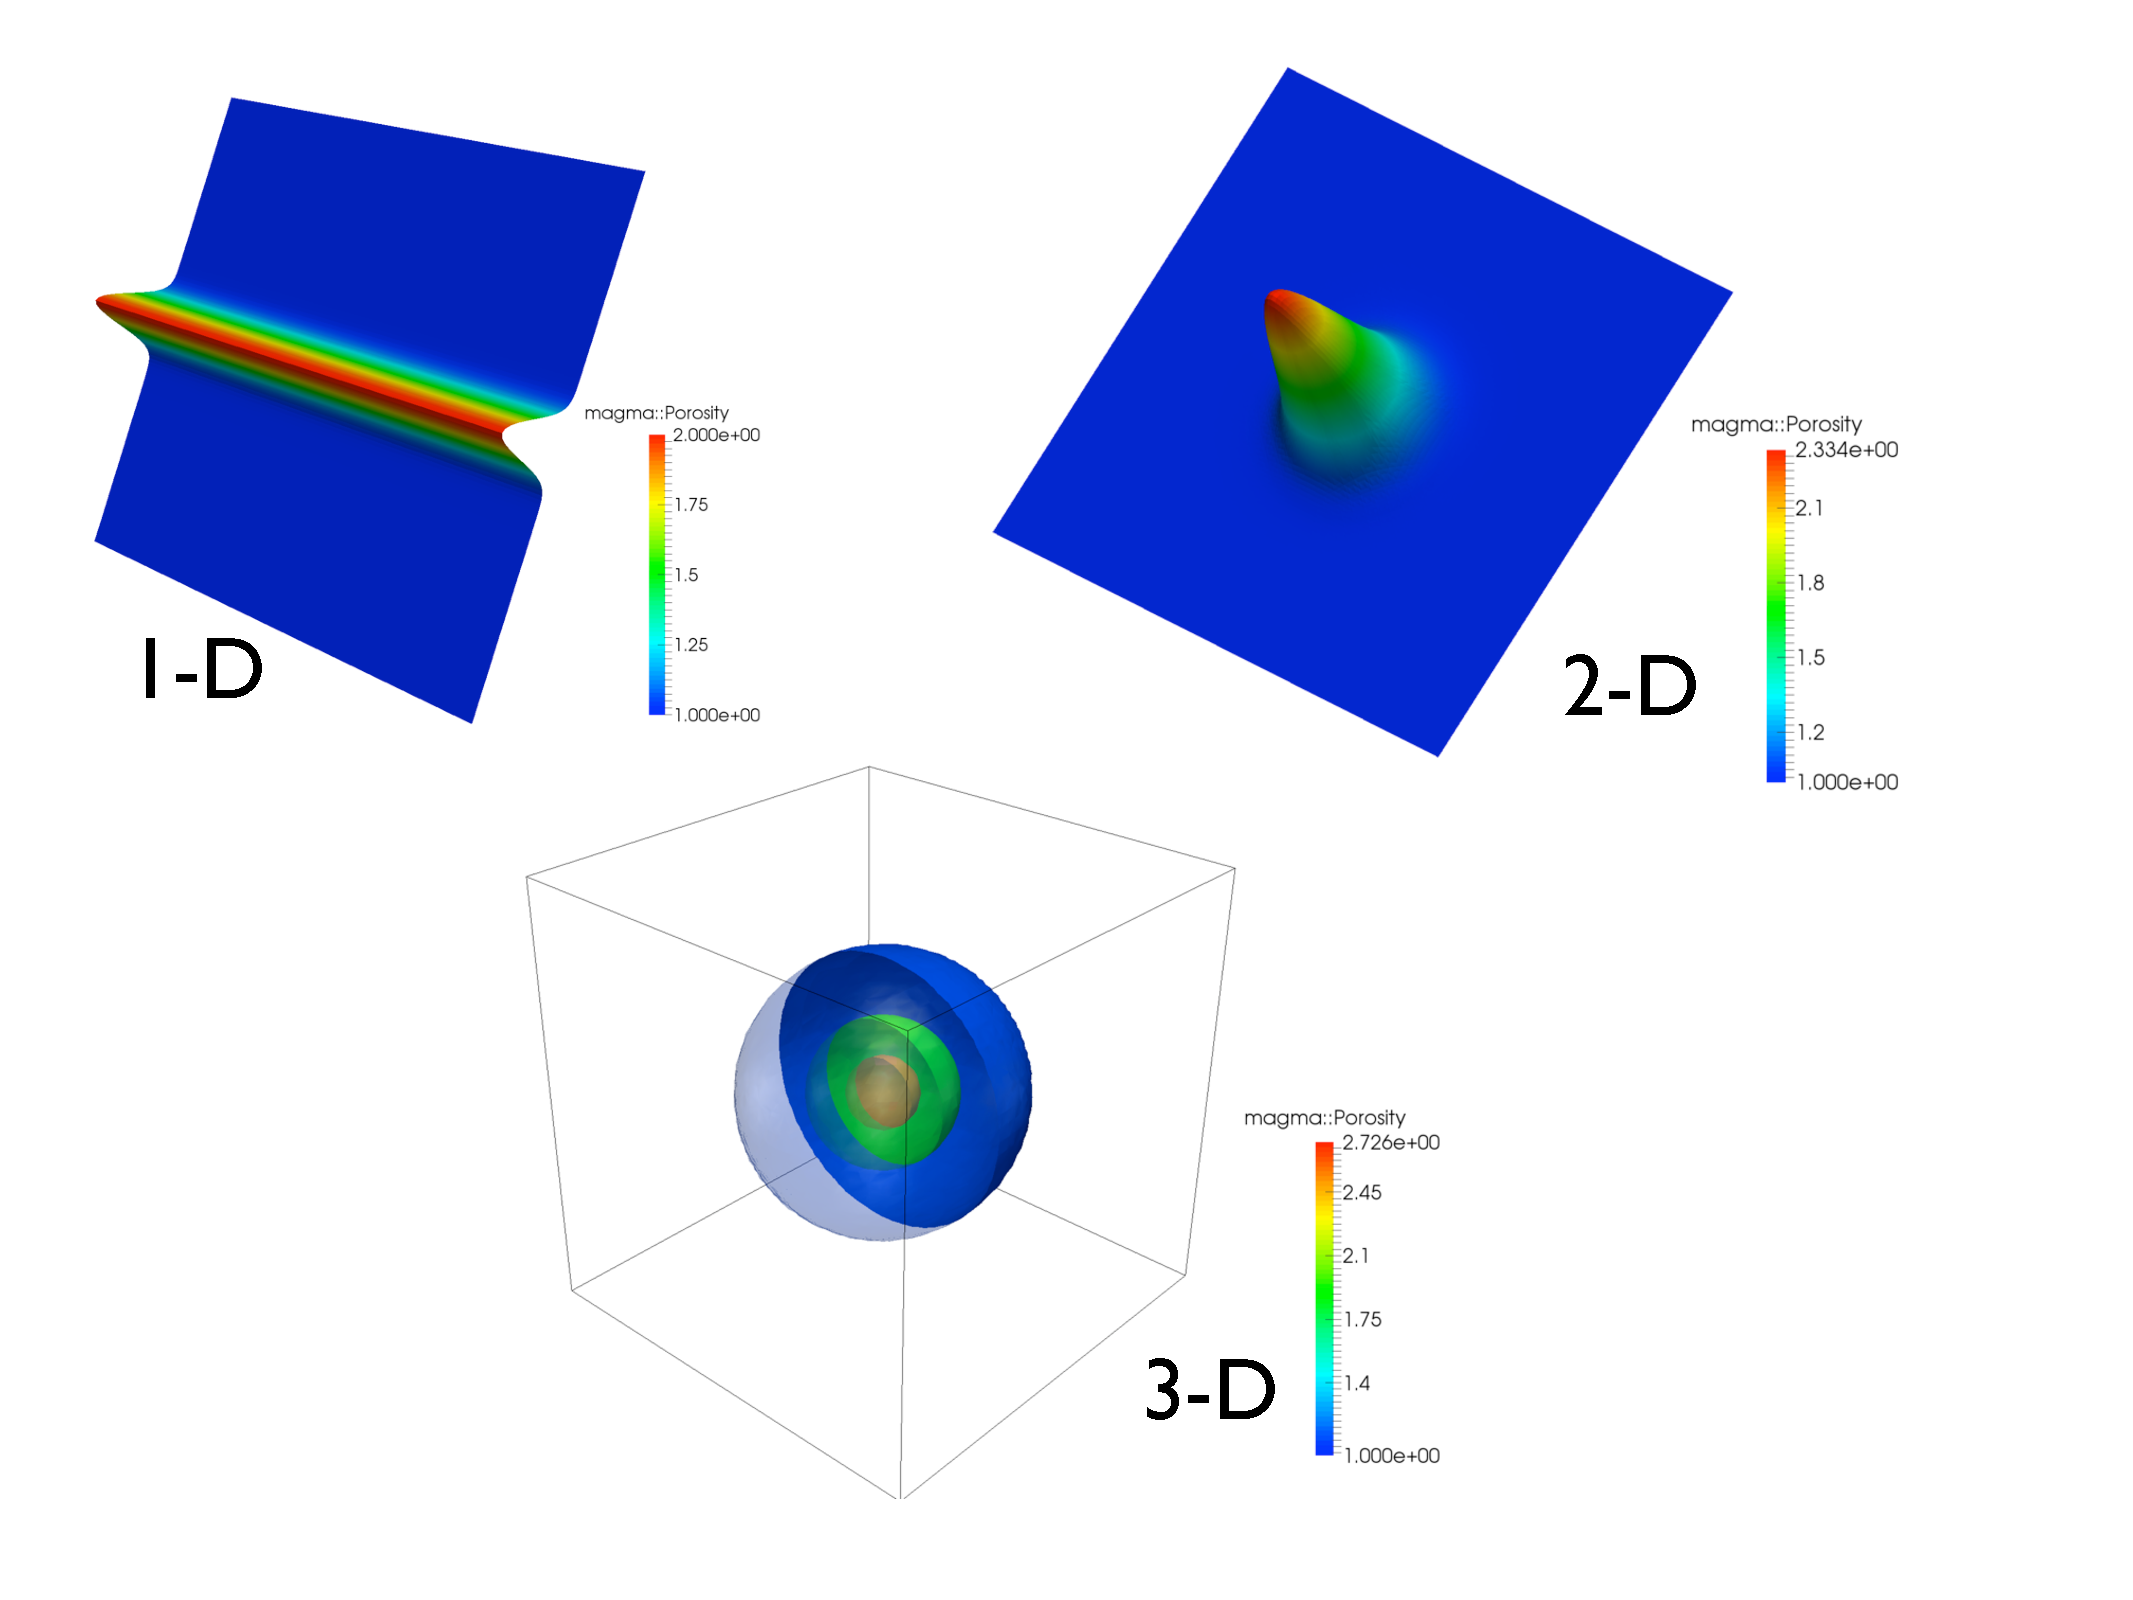
\includegraphics[width=.8\textwidth]{figures/CompositeSolitaryWaves.pdf} 
  \caption{example 1,2 and 3-D magmatic solitary waves that all move
    at speed $c=5$ times the background porosity.}
  \label{fig:SolitaryWavesAllD}
\end{figure}

In the limit of small porosity, the dimensionless governing equations for evolution
of porosity $\phi$ and ``compaction pressure'' $\pcmp$ in a frame
moving at a constant velocity $\Vs$ can be written
\begin{gather}
  \ppt{\phi} + \Vs\cdot\grad\phi = 
  \left(
    \frac{h}{\delta}
  \right)^{2}\frac{\pcmp}{\zeta}  \label{eq:5.1}\\
-\div K \grad\pcmp + \left(
    \frac{h}{\delta}
  \right)^{2}\frac{\pcmp}{\zeta} = \div K \ghat    \label{eq:5.2}
\end{gather}
where $K=\phi^{n}$ is the permeability, $\zeta = 1/\phi^{m}$ is the
bulk viscosity, $\ghat$ is the unit vector in the direction of
gravity, and $(h/\delta)$ is the system height $h$ in compaction lengths
\begin{gather}
  \delta = \sqrt{\frac{K_{0}\zeta_0}{\mu}}
\end{gather}
which is the intrinsic viscous length scale at the background
porosity.  



\subsection{Variational forms}
\label{sec:variational-forms}



\section{Solution using \TF}
\label{sec:solution-using-tf}



%\pagebreak{}
\section{Themes and Variations}
\label{sec:themes-variations}


\subsection{Variable Viscosity}
\label{sec:variable-viscosity}


%%% Local Variables: 
%%% mode: latex
%%% TeX-master: "tftutorials"
%%% End: 
